In Kapitel 3 werden wir sehen, dass es möglich ist die Elementsteifigkeitsmatrix der Masse Matrix und der Laplace Bilinearform als einen Tensor umzudefinieren. Nachdem wir dies gemacht haben, werden wir die Strukturen dieses Tensors untersuchen, mit Hinblick einen einfachen Weg zu finden, die Pseudoinverse zu bestimmen. Was genau ein Tensor ist, was wir unter der Pseudoinversen eines Tensors verstehen und wie wir einen Tensor analyisieren, wird in diesem Unterkapitel beantwortet.


\begin{Definition} (Tensor) \\
Ein Tensor ist eine multidimensionale Matrix $\pmb{\mathscr{X}}  \in \mathbb{R}^{I_1 \times I_2 \times \dots \times I_N}$.
Die Ordnung ist die Anzahl der Dimensionen, in diesem Fall $N$. 
\end{Definition}

\begin{figure}[ht]
	\centering
  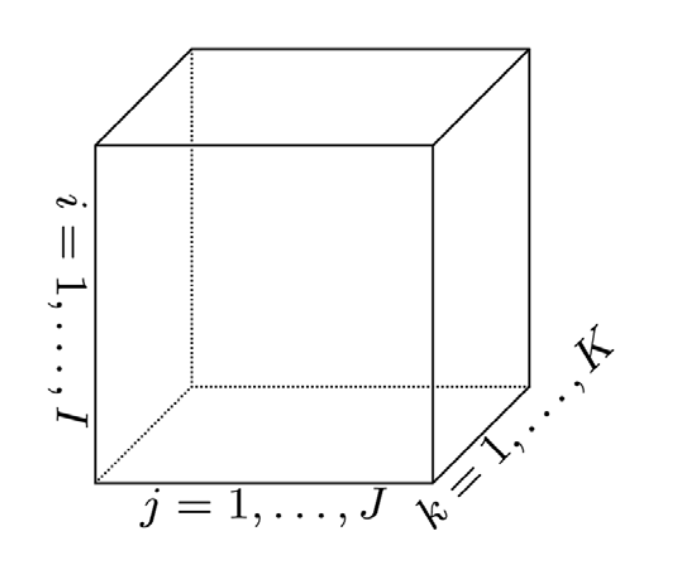
\includegraphics[width=0.3\textwidth]{tensorOrdnung3.png}
	\caption{Tensor dritter Ordnung $\pmb{\mathscr{X}}  \in \mathbb{R}^{I \times J \times K}$ \cite[456]{Kolda}}
	\label{fig:tensorOrdnung3}
\end{figure}

Vorsicht zu haben, gilt es bei den Begriffen Ordnung und Rang bei Tensoren. Es sollte vermieden werden diese Begriffe zu verwechseln. Außerdem sollte man nicht den Begriff des Rangs einer Matrix, mit dem Begriff des Ranges eines Tensors verwechseln. Die Definition des Rangs eines Tensors werden wir hier auslassen, da dies ein überaus schwieriger Begriff ist und es vermieden werden kann in dieser Arbeit damit zu hantieren. Eine ausführliche Erklärung des Begriffs finden Sie in \cite[464]{Kolda}.

\newpage

Um unsere Tensoren zu klassifizieren und charakterisieren, brauchen wir Eigenschaftsbegriffe. Es sei $\pmb{\mathscr{X}}  \in \mathbb{R}^{I_1 \times I_2 \times \dots \times I_N}$ ein Tensor.
\begin{Definition} (Symmetrie)
\begin{itemize}
\item[a)] Den Tensor $\pmb{\mathscr{X}}$ nennt man kubisch genau dann wenn $I_i = I_j$ für alle $i,j$.
\item[b)] Einen kubischen Tensor nennt man supersymmetrisch genau dann wenn die Elemente des Tensors konstant bleiben unter jeglicher Permutation der Indizes.
\item[c)] Einen Tensor nennt man stückweise symmetrisch, wenn die Elemente konstant bleiben unter der Permutation von mindestens 2 Indizes.
\end{itemize}
\end{Definition}

\begin{Definition} (Diagonal) \\
Den Tensor $\pmb{\mathscr{X}}$ nennt man diagonal, wenn
$\, x_{ \, i_1 \,, \, \dots \, , \, i_N \, } \, \neq 0$ genau dann wenn \\ $\, i_1 = \dots = i_N$.
\end{Definition}

\begin{Definition} (Faser) \\
Eine Faser ist das multidimensionale Analog zu Matrixspalten und Matrixzeilen. Wir definieren eine Faser, indem wir jeden Index abgesehen von einem festhalten.
\end{Definition}

Einen Tensor kann man entfalten. Dies impliziert eine Neuordnung der Tensorelemente in eine Matrix.
Wir betrachten nur die sogenannte \textit{mode-n Entfaltung}, da dies die einzig relevante Form der Entfaltung für uns ist.

\begin{Bemerkung} (Entfaltung) \\
Eine mode-n Entfaltung des Tensors $\pmb{\mathscr{X}}$ wird mit $\bold{X}_{(n)}$ geschrieben und ordnet die mode-n Fasern in die Spalten der Ergebnismatrix.
Formal ist es eine Abbildung des Indize N-tupels $(i_1,\dots,i_N)$ auf Matrixindizes $(i_n,j) $
\begin{equation}
j=1+\sum_{\substack{k=1 \\ k \neq n}}^{N} (i_k-1)J_k \text{ mit } J_k = \prod_{\substack{m=1 \\ m \neq n}}^{k-1} I_m
\end{equation}
\end{Bemerkung}

Nun fehlt uns noch eine Tensor Multiplikation um mit der Dekomposition von Tensoren anzufangen. 

\begin{Definition} (n-mode Produkt) \\
Das n-mode Produkt des Tensors $\pmb{\mathscr{X}}$ mit einer Matrix $\bold{U} \in \mathbb{R}^{J \times I_n}$ wird als $\pmb{\mathscr{X}} \times_n \bold{U}$ notiert. Die Ergebnismatrix hat die Größe $I_1 \times \dots I_{n-1} \times J \times I_{n+1} \times \dots I_N$
\begin{equation}
	(\, \pmb{\mathscr{X}} \times_n \bold{U} \, )_{\, i_1 \, \dots \, i_{n-1} \, j \, i_{n+1}\, \dots \, i_N} = \sum_{i_n = 1}^{I_n} x_{\, i_1 \, \dots \, i_N} \, u_{j \, i_n}
\end{equation}
\end{Definition}

\begin{Bemerkung}
Jedes mode-n Produkt kann mit Hilfe von entfaltenen Tensoren äquivalent ausgedrückt werden.
\begin{equation}
\pmb{\mathscr{Y}} = \pmb{\mathscr{X}} \times_n \bold{U} \Longleftrightarrow \bold{Y}_{(n)} = \bold{U} \bold{X}_{(n)}
\end{equation}
\end{Bemerkung}

\subsubsection{Singulärwertzerlegung höherer Ordnung}

Die \textit{Singulärwertzerlegung höherer Ordnung} bzw. \textit{Higher Order Singular Value Decomposition} (HOSVD) oder auch bekannt unter der Tucker Dekomposition ist eine uminterpretierte multidimensionale Hauptkomponentenanalyse. Man versucht durch Hauptachsentransformationen die Korrelation zwischen den verschiedenen Komponenten durch Überführung in eine neue Basis zu minimieren. 
Die HOSVD zerlegt den Tensor in einen sogenannten \textit{Core Tensor} multipliziert mit einer Matrix in jeder Ordnung. 

Allgemein ist die HOSVD des Tensors $\pmb{\mathscr{X}}  \in \mathbb{R}^{I_1 \times I_2 \times \dots \times I_N}$ gegeben durch
\begin{equation}
\pmb{\mathscr{X}}= \pmb{\mathscr{G}} \times_1 \, A^{(1)} \, \dots \, \times_N A^{(N)}
\end{equation}

Man kann äquivalent die HOSVD auch mit entfalteten Tensoren wie folgt angeben
\begin{equation}
\bold{X}_{(n)} = A^{(n)} \, \bold{G}_{(n)} \, ( \, A^{(N)} \, \otimes  \, \dots \, \otimes \, A^{(n+1)} \, \otimes A^{(n-1)} \otimes \dots \otimes \, A^{(1)} \, )^{T}
\end{equation}

\begin{Beispiel} (HOSVD Tensor dritter Ordnung) \\
Es sei $\pmb{\mathscr{X}} \in \mathbb{R}^{I \times J \times K}$.  Dann kann man den Tensor $\pmb{\mathscr{X}}$ zerlegen in 
\begin{equation}
{\pmb{\mathscr{X}}} \approx  \pmb{\mathscr{G}}  \times_1 A \times_2 B \times_3 C 
\end{equation}

wobei $A \in \mathbb{R}^{I \times P}$, $B \in \mathbb{R}^{J \times Q}$ und $C \in \mathbb{R}^{K \times R}$ die Faktormatrizen sind, welche orthogonal sind.
${\cal G}$ bezeichnet den Core Tensor und zeigt wie hoch die Korrelation zwischen den verschiedenen Komponenten ist.

\end{Beispiel}
\begin{figure}[ht]
	\centering
  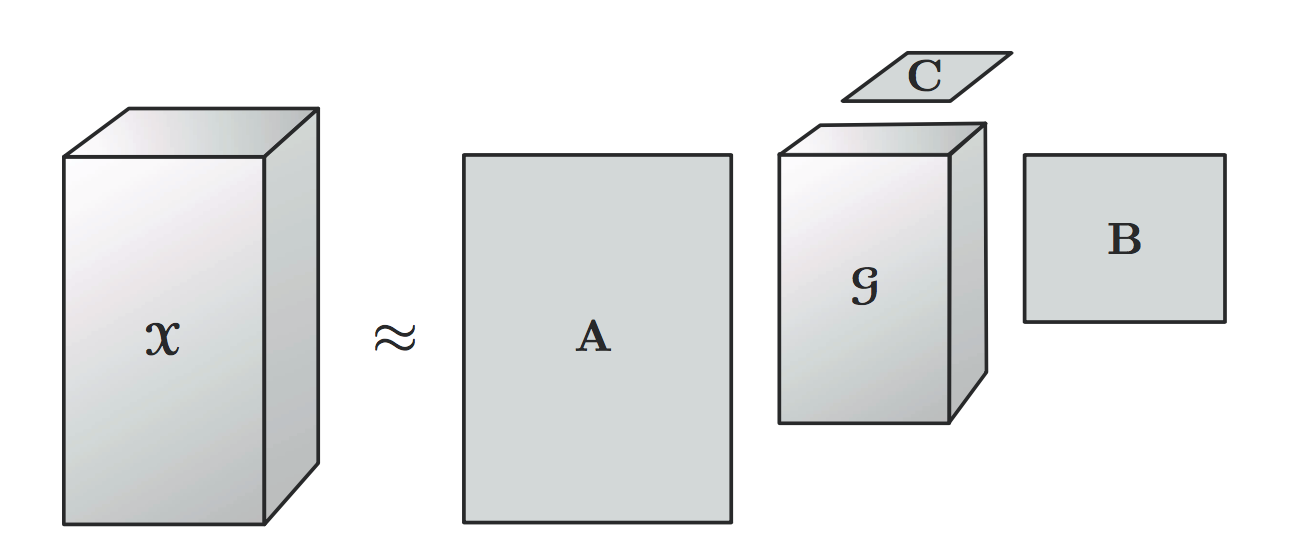
\includegraphics[width=0.6\textwidth]{hosvdTensor.png}
	\caption{HOSVD eines Tensors dritter Ordnung \cite[475]{Kolda}}
	\label{fig:hosvdTensor}
\end{figure}

\newpage
\begin{framed}
\begin{Bemerkung} (Berechnung der HOSVD) \\
Die Berechnung der HOSVD von ${\pmb{\mathscr{X}}}  \in \mathbb{R}^{I_1 \times I_2 \times \dots \times I_N}$ geht wie folgt
\begin{enumerate}
\item Berechne die mode-k Entfaltungen $\bold{X}_{(k)}$ für alle k
\item Berechne die Singulärwertzerlegung $\bold{X}_{(k)}=U_k \Sigma_k V_k^T$ und speichere $U_k$
\item Der Kerntensor ${\pmb{\mathscr{G}}} $ ergibt sich aus der Projektion des Tensors auf die Tensorbasis geformt von den Faktormatrizen  $ \, \{ \, U_k \, \}_{k=1}^{N}$  also $\, \, {\pmb{\mathscr{G}}} ={\pmb{\mathscr{X}}}  \times_{n=1}^{N} \, U_n^T$
\end{enumerate}
\end{Bemerkung}
\end{framed}

Die HOSVD existiert für alle Tensoren. Wie sieht es aber mit der Eindeutigkeit aus? Die HOSVD ist keine eindeutige Zerlegung. Dies führen wir an einem Tensor dritter Ordnung an.

\begin{Beispiel} (Eindeutigkeit der HOSVD) \\
Es seien $U \in \mathbb{R}^{P \times P}$, $V \in \mathbb{R}^{Q \times Q}$  und $W \in \mathbb{R}^{R \times R}$ . Es gilt
\begin{equation}
{\pmb{\mathscr{X}}} = {\pmb{\mathscr{G}}} \times_1 A \times_2 B \times_3 C = ({\pmb{\mathscr{G}}} \times_1 U \times_2 V \times_3 W) \times_1 AU^{-1} \times_2 BV^{-1} \times_3 CW^{-1}
\end{equation}
\end{Beispiel}

In anderen Worten: Wir können den Core Tensor ${\pmb{\mathscr{G}}}$ modifizieren, ohne die Gleichung zu ändern, solange wir das Inverse der Modifizierung auf den zugehörigen Faktormatrizen multiplizieren.

Mit dieser Kenntniss können wir nun zum Beispiel versuchen, soviele Elemente des Kerntensor wie möglich auf Null zu bekommen oder so klein wie möglich zu machen, damit wir bei der späteren Herleitung der Pseudoinversen weniger Probleme bekommen. 

Wir brauchen noch einige Eigenschaften des Kronecker Produkts, die wir uns später für die Berechnung der Pseudoinversen zu Nutze machen wollen.

\begin{Lemma} (Invertieren des Kronecker Produkts) \\
Es seien $A \in \mathbb{R}^{i \times i}$ und $B \in \mathbb{R}^{j \times j}$ invertierbar, so ist auch $(A \otimes B)$ invertierbar. Mit der Inversen
\begin{equation*}
(A \otimes B)^{-1} = A^{-1} \otimes B^{-1}
\end{equation*}
Für die Moore Penrose Pseudoinversen gilt analog
\begin{equation*}
(A \otimes B)^{+} = A^{+} \otimes B^{+}
\end{equation*}
\end{Lemma}

\begin{Lemma} (Matrixprodukt und Kronecker Produkt) \label{lemma:prod} \\
Es seien $A,B,C,D$ Matrizen, deren Matrizenprodukte $AC$ und $BD$ definiert sind, dann gilt
\begin{equation*}
AC \otimes BD = (A \otimes B)(C \otimes D).
\end{equation*}
\end{Lemma}

Dieses Ergebnisse sind entscheidend für die Herleitung der Pseudoinversen. Die theoretische Grundlage ist nun geschaffen. Es ist Zeit sich dem Herz dieser Arbeit zu widmen, nämlich der Tensorstruktur der Elementarsteifigkeitsmatrizen und die Herleitung der Pseudoinversen.

